\documentclass[a4paper,12pt]{article}
\usepackage[utf8]{inputenc}
\usepackage{amssymb,amsmath,uniinput,graphicx,hyperref, multirow,siunitx}
\usepackage[section]{placeins}
\usepackage[ngerman]{babel}
\usepackage[left=3cm,right=3cm,top=3cm,bottom=3cm]{geometry}
\renewcommand{\familydefault}{\sfdefault}
\setlength{\belowcaptionskip}{6pt}
\hypersetup{pdfinfo = {
	Title={Versuchsprotokoll zu Positronen im Festkörper},
	Author={Knut Kiesel, Tobias Pook},
	Keywords={Teilchenfalle}
}}


\graphicspath{ {../pictures/} }
\title{Laborpraktikum Teilchenphysik\\ Lebensdauer von Positronen im Festkörper}
\author{Knut Kiesel\\Tobias Pook}
\date{\today}

\begin{document}
\maketitle
\vspace{5cm}
\tableofcontents
\thispagestyle{empty}
\newpage
\setcounter{page}{1}

\section{Ziel des Versuches}
Ziel des Versuches ist der Aufbau und die Inbetriebnahme einer Messstation,
die in der Lage ist die Lebensdauer von Positronen in Festkörpern in der
Größenordnung von $\si{ps}$ zu messen.

Hierzu wird $^{22}$Na verwendet, welches beim Zerfall in $^{22}$Ne
zuerst ein γ-Quant der Energie $1.28\si{MeV}$ abgibt und dann ein Positron emittiert.
Nach einer vom Festkörper abhängigen Zeit annihiliert das Positron unter Aussendung
von 2 bis 3 γ-Quanten mit einer Energie von $0.511\si{keV}$.
Durch das messen der Zeitdifferenz zwischen dem ersten γ-Quant des Übergangs und dem
γ aus der Annihilation kann die Lebensdauer des Positrons bestimmt werden.



\section{Aufbau und Durchführung}
%Kommentare aus der Vorbesprechung:
%	Constant Fraction Discriminator liefert logisches out bei BLD Ausgang
%	Die Delay Einheit ändert die polarität des Signal, wenn gewünscht.
%	Der Multi Channel Analyzer nimmt nur positive Signal ohne Offset an.
\begin{figure}[htb]
		\centering
		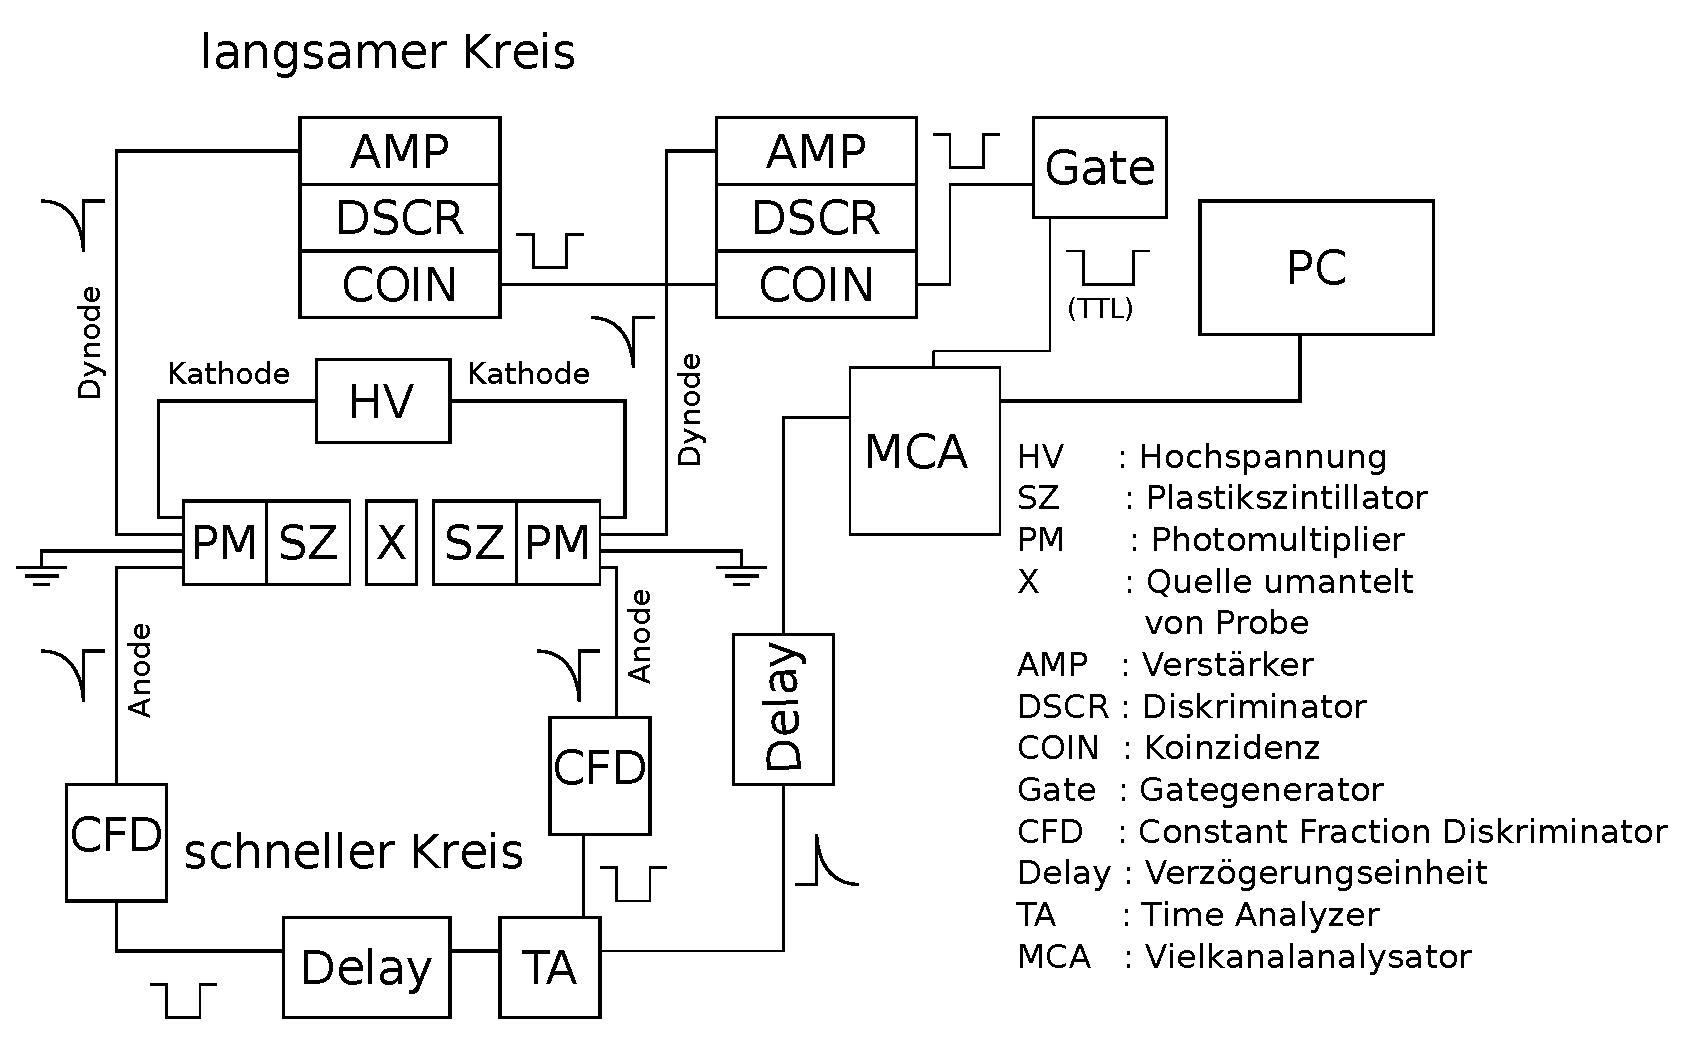
\includegraphics[width=1.0\textwidth]{../pictures/Schaltplan_custom.pdf}
		\caption{Schaltplan}
		\label{fig:schaltplan}
\end{figure}
Der Detektor besteht aus zwei zylindrischen Szintiallatonsdetektoren,
 welche in einem Gehäuse mit einem Photomultiplier verbaut sind. Die radioaktiven Proben werden zwischen beiden Szintillatoren
platziert. Die Photomultiplier werden mit einer Spannung von $2\si{kV}$ betrieben. Von beiden Photomultipliern
wird sowohl das Anodensignal als auch das Dynodensignal abgegriffen und für das Messen und Triggern der 
Zeitabstandsmessung genutzt. Hierbei liefert jeweils ein Photomultiplier das Start und der andere 
das Stoppsignal.
Die elektronische Signalverabreitung unterteilt sich in zwei Schaltkreise
 (siehe Abbildung \ref{fig:Schaltplan} für eine Blockdarstellung des gesmaten Schaltplan): \\
\begin{itemize}
	\item
	Ein "langsamer Kreis" prüft ob die gemessenen Photonen sich im richtigen Energieintervall 
	befinden und erzeugt abhängig davon ein Triggersignal.
	\item Ein "schneller Kreis" bestimmt die Zeitdifferenz und gibt dieses in Form eines Pulses an einen
	Vielkananlanalysator weiter, sofern ein Triggersignal vom "langsamen Kreis" besteht.	
\end{itemize}
\subsection*{langsamer Kreis}
	Für den langsamen Kreis wird das Dynodensiganl der Photomultiplier genutzt und in jeweils einem 
	Einzelkanaldiskriminator (\textbf{SCA}) weiter verarbeitet, dieser verstärkt das Signal zunächst (es wird
	ein Gain von 300 eingestellt). 
	% Erklären was beim Differenzieren passiert.
	Das Dynodensignal besitzt eine ausreichende linearität zwischen Energie und Pulshöhe und es ist möglich 
	zunächst ein Energiespektrum mit Hilfe des Vielkanalanalysator aufzuzeichnen.
	Anschliessend werden die Schwellwerte im Einzeldiskriminator so eingestellt, dass nur Teilchen mit einer höheren
	Energie als der rechten Flanke des Anhilationspeak als Startsignal (Fenster 2) genutzt wird und Teilchen
	mit einer niedrigeren Energie als Stoppsignal. Zusätzlich wird für das Stoppsignal eine untere Grenze bei ???
	eingestellt um den Untergrund durch niederenergetischer Teilchen und elektronisches Rauschen des Photomultiplier
	zu reduzieren. Nachdem die Fenster für Start und Stoppsignal zunächst mit dem verstärkten Dynodensignal eingestellt sind,
	wird nun ein Ausgang der Einzelkanaldiskriminatoren genutzt, der logisches Ausgangssignal liefert.
	Über eine integrierte Koinzidenzschaltung der SCA verbunden. Wenn nun Signale von beiden SCA innerhalb des Koinzidenzzeitfenster
	gemessen werden, wird ein logisches Signal an einen Gategenerator weiergeleitet. Der Gategenenerator liefert ein Ausgangssignal, dass
	am Vielkanalanlysator das Gate zur Datennahme öffnet.
\begin{figure}
		\includegraphics[width=0.8\textwidth]{../analyse/auswahl.pdf}
		\caption{Energiespektrum von $^{22}$Na. Gemessen aus dem Dynodensignal und vorverstärkt,geglättet im Einzelkanaldiskrimnator}
		\label{fig:schaltplan}
\end{figure}


\subsection*{schneller Kreis}
	Für den schnellen Kreis wird das Anodensigal der Photomultiplier genutzt. Start und Stoppsignal werden zunächst in jeweils einem Constant
	Fraction Discriminator (\textbf{CFD}) weiter verarbeitet, dieser erzeugt durch differenzieren zunächst einen bipolaren Puls aus dessen Nulldurchgang
	ein von der Pulsform unabhängiges Zeitsignal erzeugt wird und in Form eines logischen Signal ausgegeben wird. Die Signale von beiden
	CFD werden von einem Time Analyzer verarbeitet. Der Time Analyzer erzeugt einen Puls, abhängig vom Zeitlichen Abstand von Start und Stoppsignal,
	der im VKA aufgenommen und in ein Pulshöhenspektrum umgesetzt wird. Um den schnellen und langsamen Kreis zeitlich aufeinander 
	anzupassen ist zusätzlich eine Verzögerungseinheit zwischen Time Analyzer und VKA geschaltet.
	
\section{Ergebnisse}
	\subsection{Zeitkalibration}
		Um die einzelnen Kanäle des VKA mit den entsprechenden Zeitabständen zu verknüpfen wird eine Zeitkalibration durchgeführt. Dazu werden
		mit einem Pulsgenerator Pulse mit einer Amplitude von $3\si{V}$ und einer Pulsbreite von 10ns mit einer Frequenz von $1600\si{Hz}$ erzeugt.
		Es wurde mit einem Oszilloskop sichergestellt, dass Form und Amplitude des erzeugten Puls denen aus dem Anodenausgang der Photomultiplier 
		entsprechen. Das vom Pulsgenerator ausgegebene Signal wird durch ein T-Stück geteilt. Eine Abzweigung des T-Stück wird in den für das Startsignal vorgesehene 
		CFD geleitet, die andere in eine Delayeinheit und dann in den CFD für das Stoppsignal. Vor der eigentlichen Kalibrierung wird das Delay getestet, indem
		das Signal vor und nach dem Delay nicht durch die Constant Fraction Diskriminatoren sondern durch ein Oszilloskop abgegriffen werden. Hier lässt sich erkennen,
		dass beide Signale bei ausschalten des Delay nahezu zeitgleich ankommen und in ihrer Pulsform erhalten bleiben. Es kann also ausgeschlossen werden das es zu 
		zusätzlichen Verzögerungen oder sonstige Verfälschungen des Signal durch das T-Stück und die genutzten Kabel kommt.
		Nach dem testen des Delay wird die ursprüngliche Verschaltung wieder hergestellt und die zeitlichen Abstände der logischen Signale der CFDs im Time Analyzer
		in Pulshöhen umgesetzt. Die Pulse des Time Analyzer werden an den MCA weiter geleitet, dieser wird während der Kalibrierung mit
		durchgehend geöffnetem Gate betrieben. Die Verzögerung wird am Delay in $0.5\si{ns}$ Schritten von $0\si{ns}$ bis $12\si{ns}$ erhöht, das aufgezeichnete Pulshöhenspektrum 
		ist in Abbildung \ref{fig:timepuls} dargestellt. Es wird an jeden Peak im Spektrum eine Gaußfunktion angepasst, im folgenden werden die ausgewählten Zeitpunkte mit
		dem Erwartungswert $\mu$ der angepassten Verteilung assoziiert und der Fehler auf diesen Wert als Breite des Peak $\sigma$ angenommen. Da es keine Möglichkeit gab 
		(z.B. durch Vergleich mit einem weiteren Delay) die Unsicherheit auf die genutzten Verzögerungen zu bestimmen und es auch keine Angaben zu
		den Unsicherheiten in der Betriebsanweisung des Bauteil zu finden waren wurde der Fehler auf die Verzögerung zu $0.075\si{ns}$ abgeschätzt also 
		15\% der Verzögerungsschrittweite von $0.5\si{ns}$. An die so gewonnenen Zeit-Kanal Wertepaare wird eine Funktion angepasst, mit der im folgenden 
		Kanalnummern in Zeitabstände umgerechnet werden. 
		
		\begin{figure}
		\includegraphics[width=0.8\textwidth]{../analyse/peaksToArray.pdf}
		\caption{Pulshöhenspektrum zur Zeitkalibration. Die Pulse haben einen Abstand von $0.5\si{ns}$}
		\label{fig:timepuls}
		\end{figure}
\subsection{Zeitnullpunkt und Zeitstabilität}
		\begin{figure}
		\includegraphics[width=0.8\textwidth]{../analyse/compareCo.pdf}
		\caption{Gemessenes Pulshöhenspektrum für $^{60}$Co vor und nach den $^{22}$Na Messungen}
		\label{fig:timepuls}
		\end{figure}
		Zur Bestimmung des Zeitnullpunkt und zum überprüfen der zeitlichen Stabilität werden Messungen mit $^{60}$Co durchgeführt, dieses Cobaltisotop liefert 
		beim Kaskadenzerfall in $^{60}$Co zwei zeitgleiche γ-Quanten mit Energien von $1,17\si{MeV}$ und $1,33\si{MeV}$. Es wird jeweils eine Messung vor Beginn
		und nach der Hauptmessreihen mit $^{22}$Na durchgeführt. Die Ergebnisse beider Messungen sind in Abbildung \ref{fig:compare_co} dargestellt.
		Da von einem Zeitgleichen eintreffen beider Pulse ausgegangen wird, dient die Position des beobachteten Peak im Pulshöhenspektrum als Zeitnullpunkt. Es
		ist zu erkennen das sich die Position des Peakmaximum während der Versuchdurchführung um 178 Kanäle verschoben hat. Diese Verschiebung entspricht einer
		Zeitdifferenz von lediglich xx ns. Die Änderung ist also im Rahmen der Messgenauigkeit klein genug um den Mittelwert der
		beiden gemessenen Peakpositionen , Kanal 4721 , als Nullpunkt für die Zeitmessungen zu benutzen. Die Veränderung des Nullpunkt wird im folgenden
		als zusätzlich systematische Unsicherheit auf alle Zeitmessungen angenommen.  
\subsection{Vergleich der Messungen für Aluminum und Polyethylen}

\subsection{Bestimmung der Lebensdauern in Polyethylen}
		
\subsection{Globaler Fit}
Die Fitfunktion für den globalen Fit, mal schau ob das noch was wird
\begin{align*}
	F(t) &= \frac{1}{2τ} \exp\left( \frac{2}{τ}\left( μ-t+\frac{σ^2}{τ} \right) \right) \frac{2}{\sqrt{π}}\inf_{\frac{1}{\sqrt{2}σ}\left( μ-\frac{2σ^2}{τ} -t \right)}^\infty dγ e^{-γ^2}
	= \frac{1}{2τ} \exp\left( \frac{2}{τ}\left( μ-t+\frac{σ^2}{τ} \right) \right) Erfc\left(\frac{1}{\sqrt{2}σ}\left( μ-\frac{2σ^2}{τ} -t \right)\right)
\end{align*}
\section{Diskussion}

 
\section{Diskussion} 
\end{document}
